\setchaptergraphic{
    % Cauchy sequence convergence
    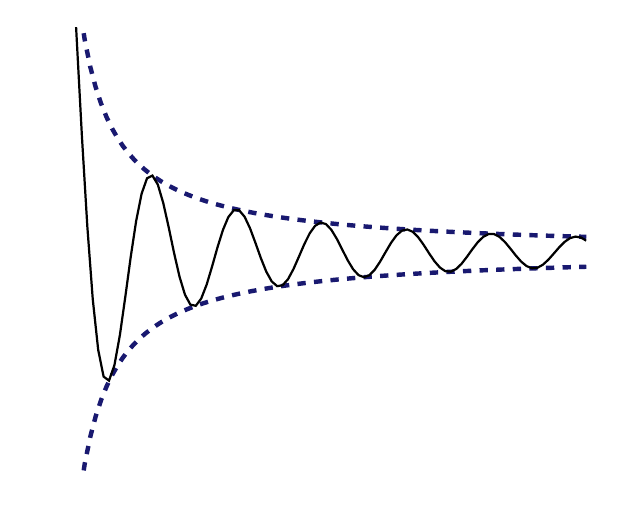
\begin{tikzpicture}[scale=1.0]
        \begin{axis}[
            xmin=0,xmax=20,
            ymin=-0.75,ymax=0.75,
            axis line style={draw=none},
            tick style={draw=none},
            xticklabels=\empty,
            yticklabels=\empty,
        ]
            \addplot[domain=0:20, MidnightBlue, dashed, ultra thick, samples=100] {+1/x};
            \addplot[domain=0:20, MidnightBlue, dashed, ultra thick, samples=100] {-1/x};
            \addplot[domain=0.1:20, black, thick, samples=100] {sin(deg(2*x))/x};
        \end{axis}
    \end{tikzpicture}
}

\chapter{Analysis}
\label{ch:analysis}

\section{Fields}

\begin{defn}
    A \emph{field} $(F, +, \cdot)$ is a set $F$ equipped with two binary operations called addition ($+$) and multiplication ($\cdot$), which do not necessarily correspond to addition and multiplication on the real numbers.

    Field axioms:
    \begin{itemize}
        \item Addition and multiplication are commutative.
        \item Addition and multiplication are associative.
        \item Additive and multiplicative identities, denoted $0$ and $1$ respectively.
        \item Every element $x \in F$ has an additive inverse denoted $-x$.
        \item Every element $x \in F$ where $x \neq 0$ has a multiplicative inverse denoted $x^{-1}$ or $1/x$.
        \item Multiplication is distributive over addition.
    \end{itemize}
\end{defn}

\begin{thm}{Field properties}\label{field-properties}\proofbreak
    For every $x, y, z \in F$:
    \begin{enumerate}
        \item $0 \cdot x = 0$
        \item $(-1) \cdot x = -x$
        \item $-(-x) = x$
        \item If $x \neq 0$, $\left(x^{-1}\right)^{-1} = x$
        \item $x \cdot (-y) = -(x\cdot y)$
        \item $(xy)^{-1} = x^{-1}y^{-1}$
        \item $x\cdot(y-z) = x\cdot y - x \cdot z$
        \item $-(x - y) = y - x$
    \end{enumerate}
\end{thm}

\begin{proof}\proofbreak
    \begin{enumerate}
        \item $0 \cdot x + 0 \cdot x = (0 + 0) \cdot x = 0 \cdot x$. Since the additive identity is unique, this implies that $0 \cdot x = 0$.
        \item $(-1) \cdot x + x = (-1) \cdot x + 1 \cdot x = (-1 + 1) \cdot x = 0 \cdot x = 0$. Therefore, $(-1) \cdot x = -x$.
        \item Let $w = -x$, then $x + w = 0$. Therefore, $x = -w$, and so $x = -(-x)$.
        \item Let $w = x^{-1}$, then $wx = 1 = xw$, so $x = w^{-1}$. Therefore, $x = w^{-1}$, and so $(x^{-1})^{-1} = w^{-1} = w$.
        \item $x \cdot (-y) + xy = x\cdot(-y + y) = x\cdot 0 = 0$.
        \item Let $(xy)(x^{-1}y^{-1}) = (yx)(x^{-1}y^{-1}) = y(xx^{-1})y^{-1} = yy^{-1} = 1$. Since the multiplicative identity is unique, $(xy)^{-1} = x^{-1}y^{-1}$.
        \item $x \cdot (y-z) = x \cdot (y + (-1)z) = x\cdot y + x \cdot (-1)z = xy - xz$.
        \item Since $(x - y) + (y-x) = x + (-y + y) - x = x - x = 0$, we know $-(x - y) = (y - x)$.
    \end{enumerate}
\end{proof}

\begin{defn}
    Let $F$ be a field, and let $x \in F$ and $n \in Z$, $n \geq 0$. Then we recursively define
    \[x^n =
        \begin{dcases}
            1, & n = 0 \\
            x \cdot x^{n-1}, & n > 0
        \end{dcases}.
    \]
\end{defn}

\begin{defn}
    An \emph{ordered field} is a field $(F, +, \cdot)$ together with a subset $F^+ \subset F$ such that\begin{itemize}
        \item For all $x, y \in F^+$, both $x + y$ and $x \cdot y$ are in $F^+$.
        \item (Trichotomy) For all $x \in F$, exactly one of $x \in F^+$, $-x \in F^+$, and $x = 0$ is true.
    \end{itemize}
\end{defn}

If $(F, F^+)$ is an ordered field and $x \in F$, we say $x$ is positive (or $x > 0$) if $x \in F+$.

\begin{defn}
    For elements $x, y$ in an ordered field, we say $x > y$ (or $y < x$) if $x - y > 0$, and $x \geq y$ (or $y \leq x$) if $x = y \lor x > y$.
\end{defn}

\begin{thm} For all $x, y, z, w \in F$, where $F$ is an ordered field:
    \begin{enumerate}
        \item $(x < y) \land (y < z) \implies (x < z)$.
        \item $(x < y) \land (z < w) \implies x + z < y + w$.
        \item $(x > 0) \land (y < 0) \implies xy < 0$.
        \item $(x < 0) \land (y < 0) \implies xy > 0$.
        \item $x \neq 0 \implies x^2 > 0$.
    \end{enumerate}
\end{thm}

\begin{proof}\proofbreak
    \begin{enumerate}
        \item $x < y \land y < z$ implies that $y - x > 0$ and $z - y > 0$. Therefore, $(y - x) + (z - y) = z - x > 0$, so $x < z$.
        \item $x < y \land z < w$ implies that $y - x > 0$ and $w - z > 0$. Therefore, $(y - x) + (w - z) = (y + w) - (x + z) > 0$, so $x + z < y + w$.
        \item $(x > 0) \land (y < 0)$ implies that $-y > 0$. Since $x(-y) > 0$ and $x(-y) = -(xy)$, it follows that $xy < 0$.
        \item $(x < 0) \land (y < 0)$ implies that $(-x)(-y) > 0$. Since $(-x)(-y) = -(-xy) = -(-xy) + (xy  + (-xy)) = (-xy) - (-xy) + xy = 0 + xy = xy$, it follows that $xy > 0$.
        \item If $x > 0$, then $x^2 > 0$. If $x < 0$, then $-x > 0$, so $(-x)^2 > 0$. Since $(-x)(-x) = x^2$, it follows that $x^2 > 0$.
    \end{enumerate}
\end{proof}

\begin{prop}\label{trichotomy-exclusion}
    Let $(F, F^+)$ be an ordered field, and $x, y \in F$. Then at most one of the following is true: $x < y$, $x > y$.
\end{prop}

\begin{proof}
    For the sake of contradiction, assume that $x < y$ and $y > x$. Since $x < y$, we know $y - x > 0$, so $(y - x) \in F^+$. Since $x > y$, we know that $y - x < 0$, so $(y - x) \in F^-$. This contradicts trichotomy, $x < y \land y > x$ cannot be true.
\end{proof}

\begin{prop}\label{greater-than-ratio}
    Let $(F, F^+)$ be an ordered field, and let $x, y \in F^{+}$. Then $x > y$ if and only if $\frac{x}{y} > 1$.
\end{prop}

\begin{proof}\proofbreak
    ($\implies$) If $x > y$, by definition $x - y > 0$. Therefore, $\frac{x}{y} - \frac{y}{y} > 0$, so $\frac{x}{y} - 1 > 0$. This implies that $\frac{x}{y} > 1$.

    ($\impliedby$) If $\frac{x}{y} > 1$, we know that $\frac{x}{y} - 1 > 0$, so it follows that $x - y > 0$. Therefore, we have $x > y$.
\end{proof}

\begin{prop}\label{average-in-between}
    Let $F$ be an ordered field, and $x, y \in F$ with $x < y$. Then $x < \frac{x+y}{2} < y$.
\end{prop}

\begin{proof}
    Since $x < y$, we know that $x + x < x + y$, so $(x + y) - 2x > 0$. Then $\frac{x+y}{2} - x > 0$, so $x < \frac{x+y}{2}$. Similarly, since $x < y$ we know that $x + y < y + y$, so $2y - (x + y) > 0$. Then we have $y - \frac{x + y}{2} > 0$, so $\frac{x + y}{2} < y$. Therefore, $x < \frac{x+y}{2} < y$.
\end{proof}

\begin{prop}\label{multiplicative-inequality-one}
    Let $F$ be an ordered field, and let $a, b, x \in F^+$ such that $a < b$. Then $ax < bx$.
\end{prop}

\begin{proof}
    Since $a < b$, by definition $b - a > 0$. Since $x > 0$, it follows that $x(b-a) > 0$, and so $xb - xa > 0$. Therefore, $ax < bx$ by definition.
\end{proof}

\begin{prop}\label{multiplicative-inequality-two}
    Let $F$ be an ordered field, and let $a, b, c, d \in F^+$ such that $a < b$ and $c < d$. Then $ac < bd$.
\end{prop}

\begin{proof}
    By Proposition \ref{multiplicative-inequality-one}, we know that $ac < bc$, and similarly that $bc < bd$. It follows by transitivity that $ac < bd$.
\end{proof}

\begin{prop}\label{square-is-positive-or-zero}
    Let $F$ be an ordered field, and $x \in F$. Then $x^2 \geq 0$, and $x^2 = 0$ if and only if $x = 0$.
\end{prop}

\begin{proof}
    If
    \begin{itemize}
        \item $x = 0$, then $x^2 = 0(0) = 0$,
        \item $x > 0$, then $x^2 \in F^+$, and so $x^2 > 0$,
        \item $x < 0$, then $(-x)^2 \in F^+$, and since $(-x)^2 = (-1)^2x^2 = x^2$, it follows that $x^2 > 0$.
    \end{itemize}
\end{proof}

\section{Real Numbers}

\begin{defn}
    A \emph{sequence} in a set $X$ is a function $f: \Z_{\geq k} \to X$.
\end{defn}

\begin{exmp}
    Let $f: \Z_{\geq 3} \to Q$ be the function given by $f(n) = \frac{(-1)^n}{n}$.
\end{exmp}

\begin{defn}
    Let $F$ be an ordered field, and $f$ a sequence in $F$. Then we say that $f$ \emph{converges} to some \emph{limit} $x \in F$ if, for every open interval $(a, b) \in F$ containing $x$, there exists $N \in Z_{\geq k}$ such that $f(n) \subseteq (a, b)$ for every $n \geq N$.
\end{defn}

\begin{thm}
    If a sequence $f$ in an ordered field $F$ is convergent, it has a unique limit.
\end{thm}

\begin{proof}
    Assume that a convergent sequence $f$ converges to two distinct limits, $L_1, L_2 \in F$. Since $L_1 \neq L_2$, one must be greater than the other, so without loss of generality we will assume that $L_1 < L_2$. By Proposition \ref{average-in-between}, we know that $L_1 < \frac{L_1+L_2}{2} < L_2$. Construct the open intervals $I_1 = (L_1 - 1, \frac{L_1+L_2}{2})$ and $I_1 = (\frac{L_1+L_2}{2}, I_2 + 1)$. Since $f$ converges to both $L_1$ and $L_2$, there must exist some $N_1, N_2 \in \Z$ such that for all $n \geq N_1$ we have $f(n) \in I_1$, and for all $n \geq N_2$ we have $f(n) \in I_2$. Now let $N$ be the largest of $N_1$ and $N_2$. For any $n \geq N$, we have $f(n) \in I_1$ so $f(n) < \frac{L_1+L_2}{2}$, and for any $n \geq N$, we have $f(n) \in I_2$ so $f(n) > \frac{L_1+L_2}{2}$. By Proposition \ref{trichotomy-exclusion}, this is a contradiction, so it must be that $f$ has a distinct limit.
\end{proof}

\begin{defn}
    A \emph{binary search sequence} in an ordered field $F$ is $\left\{[a_n, b_n]\right\}_{n \geq k}$ with $a_n, b_ \in F$ satisfying $[a_{n+1}, b_{n+1}] \subseteq [a_n, b_n]$ and $b_{n+1}-a_{n+1} = \frac{1}{2}(b_n - a_n)$.
\end{defn}

\begin{defn}
    A binary search sequence \emph{converges} to some $x \in F$ if for all $n \geq k$, $\left\{[a_n, b_n]\right\}$ contains $x$.
\end{defn}

\begin{defn}
    An ordered field $F$ is \emph{complete} if every binary search sequence converges to a unique element of $F$.
\end{defn}

\begin{defn}
    Any complete ordered field is a model for the real numbers.
\end{defn}

\begin{rmk}
    Any two complete ordered fields are isomorphic.
\end{rmk}

\begin{thm}\label{archimedean-property}
    The Archimedean property states that for any $x, y \in \R^{+}$, there exists $n \in \Z_{\geq 1}$ such that $nx > y$.
\end{thm}

\begin{proof}
    For the sake of contradiction, assume there exists some $x, y \in \R^{+}$ such that there is no $n \in \Z$ such that $nx > y$. Therefore, there is some $z \in \R$ where $z = y/x$ such that $z \geq n$ for all $n \in \Z$. Since $2^k \in \Z$ for all $k \in \Z$, it follows that $\frac{z}{2^k} \geq 1$ by Proposition \ref{greater-than-ratio}.

    Now consider the binary search sequence $f(k) = \left\{[0, \frac{z}{2^k}]\right\}_{k \geq 0}$. It is clear that $0 \in f(k)$ for all $k \in \Z_{\geq 0}$, however since $\frac{z}{2^k} \geq 1$, we also have that the $1 \in f(k)$ for all $k \in \Z_{\geq 0}$. This would imply that the binary search sequence converges to both $0$ and $1$, which contradicts the definition of the real numbers, so it follows that there is no such $z \in \R$.
\end{proof}

\begin{cor}
    Suppose $x \in \R$ satisfies $0 \leq x \leq \frac{1}{n}$ for every $n \in \Z_{\geq 1}$. Then $x$ must be zero.
\end{cor}

\begin{proof}
    Assume, for the sake of contradiction, that $x \neq 0$. Then by the Archimedean property \ref{archimedean-property}, there exists $n \in \Z_{\geq 1}$ such that $nx > 1$, and so $x > \frac{1}{n}$ by Proposition \ref{greater-than-ratio}. This is a contradiction, and so $x = 0$.
\end{proof}

\begin{thm}\label{bernoullis-inequality}Bernoulli's inequality\proofbreak
    Let $n \in \Z$, $x \in \R$ such that $n \geq 0$ and $x \geq -1$. Then \[(1 + x)^n \geq 1 + nx.\]
\end{thm}

\begin{proof}
    We will proceed by induction on $n$. For $n=0$, we have $(1 + x)^0 = 1$, and $1 + 0x = 1$, and so the base case is true since $1 \geq 1$.

    Assume that $(1 + x)^n \geq 1 + nx$ for some $n \geq 0$. Then
    \begin{align*}
        (1 + x)^{n+1} &= (1 + x)(1 + x)^n \\
        &= (1 + x)^n + x(1 + x)^n.
    \end{align*}
    Since $(1 + x)^n \geq 1 + nx$, we then have
    \begin{align*}
        (1 + x)^{n+1} &= (1 + x)^n + x(1 + x)^n \\
        &\geq 1 + nx + x(1 + nx) \\
        &= 1 + (n+1)x + nx^2
    \end{align*}
    Note that $x^2 \in \R^+$ by Proposition \ref{square-is-positive-or-zero}, and so $nx^2 \geq 0$. It follows that $1 + (n+1)x + nx^2 \geq 1 + (n+1)x$. Therefore, $(1 + x)^{n+1} \geq 1 + (n+1)x$ by transitivity, and so the induction is complete.
\end{proof}

\begin{lemma}\label{geometric-progression}
    For $r \neq 1$ and $n \in \Z_{\geq 1}$, \[1 + r + r^2 + \cdots + r^{n-1} = \frac{1-r^n}{1-r}.\]
\end{lemma}

\begin{proof}
    We will prove this by induction. For the base case, let $n = 1$. Since $r^0 = 1$, and $\frac{1-r^1}{1-r} = 1$, the base case is true.

    Assume that $1 + r + r^n + \cdots + r^{n-1} = \frac{1-r^n}{1-r}$ for some $n \geq 1$. Then $1 + r + r^n + \cdots + r^{n-1} + r^n = \frac{1-r^n}{1-r} + r^n = \frac{1-r^n}{1-r} + \frac{r^n - r^{n+1}}{1-r}$, so it follows that $1 + r + r^n + \cdots + r^{n-1} + r^n = \frac   {1-r^{n+1}}{1-r}$.

    By the induction principle, it follows that the lemma is true for all $n \geq 1$.
\end{proof}

\begin{lemma}\label{freshmans-reality}
    Let $a, b \in \R$ and $n \in \Z_{\geq 1}$. Then \[b^n - a^n = (b - a)\sum_{k=0}^{n-1} b^ka^{n-1-k}.\]
\end{lemma}

\begin{proof}
    If $b = a$, then $b - a = b^n - a^n = 0$, so the lemma is true in this case.
    If $a = 0$, then $b^n - a^n = b^n$, and $(b - a)\sum_{k=0}^{n-1} b^ka^{n-1-k} = b\sum_{k=0}^{n-1}b^k = b^n$. Now assume $b \neq a$ and $a \neq 0$, and let $r = \frac{b}{a}$. Then $r \neq 1$, so $1 + r + r^2 + \cdots + r^{n-1} = \frac{1-r^n}{1-r}$ by Lemma \ref{geometric-progression}. It then follows that $r^n-1 = (r-1)\sum_{k=0}^{n-1}r^k$. Notice that $r^n - 1 = \frac{b^n}{a^n} - 1 = b^n - a^n$. Therefore, $b^n - a^n = (b-a)\sum_{k=0}^{n-1}b^ka^{n-1-k}$.
\end{proof}

\begin{lemma}\label{exponent-inequality}
    Let $a, b \in \R^+$ such that $a < b$. Then $a^n < b^n$ for all $n \in \Z_{\geq 1}$.
\end{lemma}

\begin{proof}
    We will prove this by induction on $n$. In the base case $n=1$, we have $a^1 = a$ and $b^1 = b$, and so $a^1 < b^1$.

    Assume that $a^n < b^n$ for some $n \geq 1$. Since $a < b$, it follows by Proposition \ref{multiplicative-inequality-two} that $a^n(a) < b^n(b)$ and so $a^{n+1} < b^{n+1}$.

    Therefore, $a^n < b^n$ for all $n \in \Z_{\geq 1}$.
\end{proof}

\begin{lemma}\label{harmonic-vs-powers-of-two}
    For all $n \in \Z_{\geq 1}$, $\frac{1}{2^n} < \frac{1}{n}.$
\end{lemma}

\begin{proof}
    By Proposition \ref{greater-than-ratio}, $\frac{1}{n} > \frac{1}{2^n}$ if and only if $2^n > n$. We will prove this by induction on $n$. In the base case, $n=1$, we have $2^1 = 2 > 1$.

    Assume that $2^n > n$ for some $n \geq 1$. Then
    \begin{align*}
        2^{n+1} &= 2(2^n) > 2n
        &= n + n \geq n + 1,
    \end{align*}
    so the induction is complete.
\end{proof}

\begin{thm}
    Let $n \in \Z_{\geq 1}$, and let $x \in \R^+$. Then there exists $y \in \R^+$ such that $y^n = x$. We say that $y$ is the $n$th root of $x$ in $\R^+$, and denote $y$ by $\sqrt[n]{x}$ or $x^{1/n}$.
\end{thm}

\begin{proof}\proofbreak
\textbf{Uniqueness.} Suppose $y_1, y_2 \in \R^+$ such that $y_1^n = x$ and $y_2^n = x$. By trichotomy, either $y_1 < y_2$, $y_1 = y_2$, or $y_1 > y_2$. If $y_1 < y_2$, then by Lemma \ref{exponent-inequality} it follows that $y_1^n < y_2^n$. However, this would imply that $x < x$ which is a contradiction. Similarly, $y_1 > y_2$ would imply that $x > x$, and so it must be that $y_1 = y_2$.

\textbf{Existence.} Define a sequence in $\R$ starting with $[a_0, b_0] = [0, 1 + x]$, and for $k \leq 0$ as follows.
\[
    [a_{k+1}, b_{k+1}] =
    \begin{dcases}
        \left[a_k, \frac{a_k+b_k}{2}\right], & x \leq \left(\frac{a_k+b_k}{2}\right)^n \\
        \left[\frac{a_k+b_k}{2}, b_k\right], & x > \left(\frac{a_k+b_k}{2}\right)^n
    \end{dcases}
\]

By induction, this sequence must be a binary search sequence. Note that since $a_0 = 0$, and $a_{k+1} \geq a_k$, we know that $0 \leq a_k$, and so if the sequence converges to a value, that value must be greater than or equal to zero.

Now we will show by induction on $k$ that $(a_k)^n \leq x \leq (b_k)^n$ for all $k \in \N$. In the base case, we want to show that $0^n \leq x \leq (1+x)^n$. Since $0^n = 0$ and $x \in \R^+$, we have $0^n \leq x$. Additionally, by Bernoulli's inequality \ref{bernoullis-inequality}, we have $(1+x)^n \geq 1 + nx$, and since $n \geq 1$ it follows that $(1 + x)^n \geq 1 + x > x$, and so $x \leq (1+x)^n$ as needed.

Assume that $a_k^n \leq x \leq b_k^n$ for some $k \leq 0$. If $x \leq \left(\frac{a_k+b_k}{2}\right)^n$, then $a_{k+1} = a_k$ and so $(a_{k+1})^n \leq x$ by assumption and since $b_{k+1} = \frac{a_k+b_k}{2}$, we trivially have $x \leq (b_{k+1})^n$. Similarly, if $x > \left(\frac{a_k+b_k}{2}\right)^n$ then $a_{k+1} = \frac{a_k+b_k}{2}$ and so trivially $(a_{k+1})^n \leq x$, and $x \leq (b_{k+1})^n$. Therefore, the induction is complete and so $a_k^n \leq x \leq b_k^n$ for all $k \in \N$.

By completeness, this binary search sequence converges to a value $y \in \R$ such that $y \geq 0$. Since $y \in [a_k, b_k]$ for all $k$, we know that $0 \leq a_k \leq y \leq b_k$, and so by Lemma \ref{exponent-inequality} we have $(a_k)^n \leq y^n \leq (b_k)^n$. Therefore,
\[x, y^n \in [(a_k)^n, (b_k)^n] \textrm{ for all } k.\] It follows that
\[\abs{x - y^n} \leq (b_k)^n  - (a_k)^n,\] which by Lemma \ref{freshmans-reality} is equal to
\[(b_k - a_k)\sum_{j=0}^{n-1}(b_k)^j(a_j)^{n-1-j},\] and since $a_k \leq b_k$ this is less than or equal to
\[(b_k - a_k)\sum_{j=0}^{n-1}(b_k)^{n-1} = (b_k-a_k)(n)(b_k)^{n-1}.\]
Since the sequence is a binary search sequence, $(b_k-a_k) = \frac{1}{2^k}(b_0 - a_0)$ and $b_k \leq b_0$ so $(b_k)^{n-1} \leq (b_0)^{n-1}$ by Lemma \ref{exponent-inequality}. It follows that
\[(b_k-a_k)(n)(b_k)^{n-1} \leq \frac{1}{2^k}(b_0 - a_0)(n)(b_0)^{n-1},\] and so by transitivity we have
\[\abs{x - y^n} \leq \frac{1}{2^k}(b_0 - a_0)(n)(b_0)^{n-1},\] which implies that
\[0 \leq \frac{\abs{x - y^n}}{(b_0 - a_0)(n)(b_0)^{n-1}} \leq \frac{1}{2^k}.\] Since $\frac{1}{2^k} < \frac{1}{k}$ for $k \geq 1$ by Lemma \ref{harmonic-vs-powers-of-two}, it follows that $\abs{x - y^n} = 0$ by the Archimedean property \ref{archimedean-property}, and so $y^n = x$.
\end{proof}

\begin{defn}
    Let $x \in \R^+$, and $a, b \in \Z$ with $b > 0$. We define $x^{a/b}$ be to $\left(x^{1/b}\right)^a$.
\end{defn}
